\documentclass[]{interact}

\usepackage[T1]{fontenc}
\usepackage{epstopdf}
\usepackage[caption=false]{subfig}
\usepackage{amsmath,amssymb,amsthm}
\usepackage{booktabs}

\usepackage[natbibapa]{tfapastyle}
\setlength\bibhang{12pt}
\renewcommand\bibliographytypesize{\fontsize{10}{12}\selectfont}

\usepackage{hyperref}
\usepackage{url}

\theoremstyle{plain}
\newtheorem{theorem}{Theorem}[section]
\newtheorem{lemma}[theorem]{Lemma}
\newtheorem{corollary}[theorem]{Corollary}
\newtheorem{proposition}[theorem]{Proposition}
\newtheorem{observation}[theorem]{Observation}

\theoremstyle{definition}
\newtheorem{definition}[theorem]{Definition}
\newtheorem{example}[theorem]{Example}

\theoremstyle{remark}
\newtheorem{remark}{Remark}
\newtheorem{notation}{Notation}

\begin{document}

\articletype{RESEARCH ARTICLE}

\title{Pollock Visual Algebra: Prime-Factor Drip Paintings with Homomorphic Composition and Geometric Resilience}

\author{
\name{Leonardo Ara\'{u}jo\textsuperscript{a}\thanks{CONTACT Leonardo Ara\'{u}jo. Email: leolca@ufsj.edu.br}}
\affil{\textsuperscript{a}DTECH/UFSJ --- Universidade Federal de S\~{a}o Jo\~{a}o del-Rei, Ouro Branco, MG, Brazil}
}

\maketitle

\begin{abstract}
Drawing on Jackson Pollock's drip-painting aesthetic, we develop a family of prime-factor visual representations in which each prime seeds a deterministic, velocity-coupled paint trajectory in a distinct hue. We contrast two factor-driven generative grammars (\emph{Separate Strokes} and prefix-preserving \emph{Path Extent}) with two monoid homomorphisms realizing $\Phi(a \cdot b) = \Phi(a) \star \Phi(b)$: \emph{Translucent Multiply Glazing} (TMG, exact in continuous attenuation space, with at most a $1$-LSB discrepancy across tested 8-bit RGB compositions) and \emph{Toroidal Trajectory Sum} (TTS, exact in continuous toroidal trajectory space $\mathcal{T} = C([0,1], \mathbb{T}^2)$). As a proof of concept over $1 \le n \le 120$, all four variants achieve $100\%$ exact-RGB uniqueness and template-invertibility recovery given precomputed prime templates (validating visual invertibility rather than offering an integer-factorization algorithm), with $100\%$ recovery extending across $200$ random composites in $2 \dots 10{,}000$ for Separate Strokes, Path Extent, and TMG. Finally, we extend TMG into a single-canvas $512 \times 512$ binary message codec with a keyed organic registration skein for Fourier--Mellin alignment. Across $1{,}000$-trial Monte Carlo benchmarks under rotation, translation, scaling (RTS), JPEG ($q=80$), and Gaussian noise ($\sigma=8$), uncoded $64$- and $128$-bit payloads achieve $99.74\%$--$99.76\%$ bit accuracy ($87.3\%$--$92.4\%$ exact messages), isolation ablations show geometric resampling drives virtually all errors, and adding a $\mathrm{BCH}(127,92,t=5)$ error-correcting code raises exact-message recovery to $99.00\%$ ($396/400$ trials).
\end{abstract}

\begin{keywords}
mathematical art; Jackson Pollock; prime factorization; aesthetic computing; visual homomorphism; geometric resilience
\end{keywords}

\section{Introduction}
Positive integers are abstract entities independent of any single notation \citep{menninger1969number,reimann2024visual}. Standard positional systems—such as decimal, duodecimal, sexagesimal, and binary \citep{ifrah2000universal,menninger1969number}—express a number as a sum of powers of a fixed base $b$, which makes magnitude comparison, addition, and divisibility by factors of $b$ immediate from the digits alone. However, positional digits obscure multiplicative structure outside the base: in base $10$, the consecutive numerals $14$ and $15$ look nearly identical, giving no visual cue that $14 = 2 \times 7$ and $15 = 3 \times 5$ have completely disjoint prime factors, nor that $14 \times 15 = 210$ combines the factors of $14$ and $15$.

In plain terms, the central idea is to assign each prime number a deterministic visual signature consisting of a characteristic hue and a reproducible drip trajectory. Composite integers are represented by combining the signatures of their prime factors—either layered sequentially or, in our homomorphic variants, merged as translucent glazes or summed toroidal paths—so that the resulting paintings expose multiplicative structure through overlapping organic trajectories.

Representing integers directly through \emph{prime factorization} reveals that hidden structure—fulfilling what \citet{arcavi2003role} describes as visualization's role in ``seeing the unseen'' within abstract mathematical objects, extending \citeauthor{giaquinto2007visual}'s \citeyearpar{giaquinto2007visual} account of visual thinking in arithmetic, and echoing \citet{harriss2022art} in viewing mathematical illustration as an inherently artistic mapping from abstract structure into perceptual form. By the \emph{Fundamental Theorem of Arithmetic}, every integer $n > 1$ admits a decomposition into prime numbers that is unique up to the ordering of factors:
\[
  n = \prod_{i=1}^{r} p_i^{e_i},
\]
where $p_1 < p_2 < \dots < p_r$ are distinct primes and $e_i \ge 1$ are their multiplicities (with $n = 1$ serving as the empty product, or multiplicative identity). Integer factorization and the Fundamental Theorem of Arithmetic are central to number theory \citep{hardy2008introduction} and public-key cryptography such as RSA \citep{rivest1978method} because multiplication is computationally easy while recovering prime factors is believed hard.\footnote{On classical computers; Shor's quantum algorithm factors integers in polynomial time.}

Standing at the intersection of mathematics and the arts \citep{emmer1993visual,bill1993mathematical}—and echoing \citet{goodman1968languages} on formal symbol systems and \citet{fishwick2006aesthetic} on \emph{aesthetic computing}—we aim for visual number representations that are simultaneously \emph{algebraically composable and algorithmically recoverable} yet \emph{aesthetically compelling} as visual art. Prior prime-factor visualizations, including \citet{ashwell2020prime}, Huff's 3D ``genetic'' sculptures \citep{huff2006visually}, Yorgey's recursive \emph{Factorization Diagrams} \citep{yorgey2012factorization}, \citet{reimann2024visual}, and \citet{basegmez2026symmetries}, share a common workflow: to depict a given integer $n > 1$ (prime or composite), one first computes its prime decomposition arithmetically and only then arranges visual symbols accordingly. In computational neuroscience, \citet{kleyko2022integer} take a complementary algebraic step using Vector Symbolic Architectures, binding distributed prime hypervectors so that multiplication becomes algebraic binding and factors are recovered via resonator-network unbinding; by contrast, our representations operate on deterministic 2D visual trajectories and pixel/toroidal compositions, with template-based peeling or linear log-attenuation decoding. Table~\ref{tab:lit} contrasts these approaches with the present work, separating factor-driven construction, representation-space composition, and factor recovery (noting that a representation can be compositional without being invertible, and invertible without being a homomorphism). Rather than introducing a new algebraic structure, this work investigates how the familiar monoid isomorphism $(\mathbb{N}_{>0}, \cdot, 1) \to (\mathbb{N}_{\ge 0}^{(\infty)}, +, \mathbf{0})$ sending $n$ to its finitely supported prime-exponent sequence $\mathbf{e}(n) = (e_1, e_2, \dots)$—under which $\mathbf{e}(ab) = \mathbf{e}(a) + \mathbf{e}(b)$—can be realized visually through layered drip trajectories inspired by Jackson Pollock (c.\ 1947--1950). The contributions of this work are threefold: (1)~a family of four deterministic drip-painting encodings contrasting generative grammars with monoid homomorphisms; (2)~two formal visual homomorphisms (TMG in continuous pixel attenuation space and TTS on the flat torus $\mathbb{T}^2$) with blind factor-recovery algorithms over $1 \le n \le 120$; and (3)~a single-canvas binary message codec combining TMG with an integrated organic registration skein and log-attenuation linear decoding.

\begin{table}[ht]
  \centering
  \caption{Comparison of prior prime-factor representations and the present Pollock visual algebra.}
  \label{tab:lit}
  \footnotesize
  \begin{tabular}{@{}llll@{}}
    \toprule
    Approach & Visual / Vector Medium & Composition Law & Factor Recovery \\
    \midrule
    \citet{ashwell2020prime} & Painted pattern motifs & Factor-driven placement & Visual inspection \\
    \citet{huff2006visually} & 3D generative sculptures & Factor-based construction & Structural reading \\
    \citet{yorgey2012factorization} & Recursive 2D diagrams & Recursive grouping & Structural inspection \\
    \citet{reimann2024visual} & Geometric integer patterns & Factor-driven layout & Structural reading \\
    \citet{basegmez2026symmetries} & Dihedral rosette pictographs & Factor-driven symmetry & Structural reading \\
    \citet{kleyko2022integer} & Distributed hypervectors & Algebraic vector binding & Resonator unbinding \\
    Present paper & Pollock drip trajectories & Pixel / trajectory laws & Template peeling / DFS\footnote{Requires precomputed prime templates.} \\
    \bottomrule
  \end{tabular}
\end{table}

\section{Pollock's Action Painting as a Prime-Factor Medium}
Pollock's mature drip paintings abandon a single focal center in favor of an ``all-over'' field of interwoven poured-paint trajectories, whose scaling properties were analyzed as fractal-like by \citet{taylor1999fractal}—though that fractal characterization remains debated \citep{jonessmith2006fractal}. Rapid arm motions produce thin filaments, while pauses and direction changes pool into thicker droplets and satellite splatters. Compared with rigid geometric grids or concentric emblems, continuous drip trajectories weave prime factors across the entire canvas without crowding a single center. This physical grammar maps onto prime-factor synthesis via empirical design parameters chosen for visual legibility and low inter-stroke overlap:
\begin{itemize}
  \item \textbf{Chromatic prime identity:} Let $p_0 < p_1 < p_2 < \dots$ ($2, 3, 5, \dots$) denote all primes in ascending order. Each prime $p_j$ ($j \in \{0, 1, \dots\}$) is assigned an HSL color with golden-angle hue $H(j) = (j \cdot 137.508^\circ + 18^\circ) \bmod 360^\circ$. Because $137.508^\circ$ is a $3$-decimal rational approximation to the irrational golden angle $360^\circ / \varphi^2 \approx 137.507764^\circ$ ($\varphi = (1+\sqrt{5})/2$), with $137.508 / 360 = 11459 / 30000$ in lowest terms, the palette is strictly periodic with period $30{,}000$ primes—providing a deterministic palette of $30{,}000$ distinct hue values before repetition (whereas exact irrational rotations are asymptotically equidistributed \citep{kuipers1974uniform}, hue uniqueness over $30{,}000$ steps does not guarantee perceptual distinguishability at large $j$, though short prefixes remain well dispersed). Saturation and base lightness are chosen empirically to keep pigments vivid on cream linen without approaching near-black; in opaque mode, repeated occurrences $k \in \{1, \dots, e\}$ of a prime power $p_j^e$ cycle lightness across three levels for visual separation.
  \item \textbf{Deterministic drip trajectory:} Each prime occurrence $(p_j, k)$—with $k \in \{1, \dots, e\}$ in Separate Strokes mode and $k = 1$ in Path Extent and TMG—seeds a 32-bit Mulberry32 PRNG via $(p_j \cdot c_1) \oplus (k \cdot c_2) \bmod 2^{32}$. On an $S \times S$-pixel canvas ($S = 100$ in Sections~2--4) inset by an $8\%$ border margin $m = 0.08S$, starting from $(x_0, y_0) \sim \mathcal{U}[m, S-m]^2$ with $\theta_0 \sim \mathcal{U}[0, 2\pi)$ and $v_0 \sim \mathcal{U}[0.08S, 0.22S]$, each step $t = 1, \dots, T_{\mathrm{base}}$ ($T_{\mathrm{base}} = 32$) updates:
  \begin{align}
    \theta_t &= \theta_{t-1} + \delta_\theta, \qquad \delta_\theta \sim \mathcal{U}[-0.95, 0.95]\text{~rad}, \label{eq:drip_angle} \\
    v_t &= \operatorname{clip}\!\left(v_{t-1} \cdot \delta_v,\; 0.03S,\; 0.25S\right)\text{~px/step}, \qquad \delta_v \sim \mathcal{U}[0.75, 1.30], \label{eq:drip_speed} \\
    x_t &= x_{t-1} + v_t \cos\theta_t, \qquad y_t = y_{t-1} + v_t \sin\theta_t, \label{eq:drip_pos}
  \end{align}
  with specular reflection at the margin boundaries ($\theta_t \leftarrow \pi - \theta_t$ on $x \notin [m, S-m]$, $\theta_t \leftarrow -\theta_t$ on $y \notin [m, S-m]$, clamping coordinates to $[m, S-m]$). Segments are rendered as quadratic B\'ezier curves with velocity-coupled stroke width, paint pooling at low speeds, and satellite spray droplets at high speeds (all remaining rendering constants and PRNG offsets are documented in \texttt{report\_all\_modes.pdf} and the code repository).
  \item \textbf{Identity element:} The unit $n = 1$ corresponds to the blank cream linen background $I_{\mathrm{bg}}$.
\end{itemize}

\section{Homomorphism vs.\ Generative Grammar}
Intuitively, the difference between our two design families is like following a recipe versus blending two already-cooked dishes: in a \emph{generative grammar}, you must know a number's prime ingredients before lifting the brush, whereas in a \emph{visual homomorphism}, you can take two finished paintings and combine them directly to obtain the painting of their product. Formally, let $(\mathbb{N}_{>0}, \cdot, 1)$ denote the multiplicative commutative monoid of positive integers, $\mathcal{I}$ a representation space equipped with a binary composition $\star$, and $\Phi : \mathbb{N}_{>0} \to \mathcal{I}$ a \emph{visual encoding map} \citep{dummit2003abstract}. We call $\Phi$ a \emph{visual homomorphism} (i.e., a monoid homomorphism) if $\Phi(1) = I_{\mathrm{bg}}$ and $\Phi(a \cdot b) = \Phi(a) \star \Phi(b)$ for all $a, b \in \mathbb{N}_{>0}$, where the image-space composition $\star$ is factor-blind—operating solely on the already-rendered canvases $\Phi(a)$ and $\Phi(b)$ without factoring $a \cdot b$ (whereas evaluating $\Phi(n)$ directly from $n$ still uses $n$'s prime factorization). By contrast, a \emph{generative grammar} requires the prime-factor multiset $\{p_i^{e_i}\}$ prior to rendering.

Figure~\ref{fig:modes} contrasts how these two paradigms handle prime powers ($2, 4=2^2, 8=2^3$) and composites ($6, 12=2^2\cdot 3, 30=2\cdot 3\cdot 5$). In the top two rows (generative grammars), \emph{Separate Strokes} adds $e$ distinct opaque strokes one over another, whereas \emph{Path Extent} keeps a single stroke per prime and extends its length $e$-fold along the same initial prefix. In the bottom two rows (homomorphisms), \emph{TMG} deepens a prime's translucent glaze ($A_p^e$) without opaque occlusion, while \emph{TTS} scales and sums smooth harmonic trajectories in $[0, 1)^2$.

\begin{figure}[t]
  \centering
  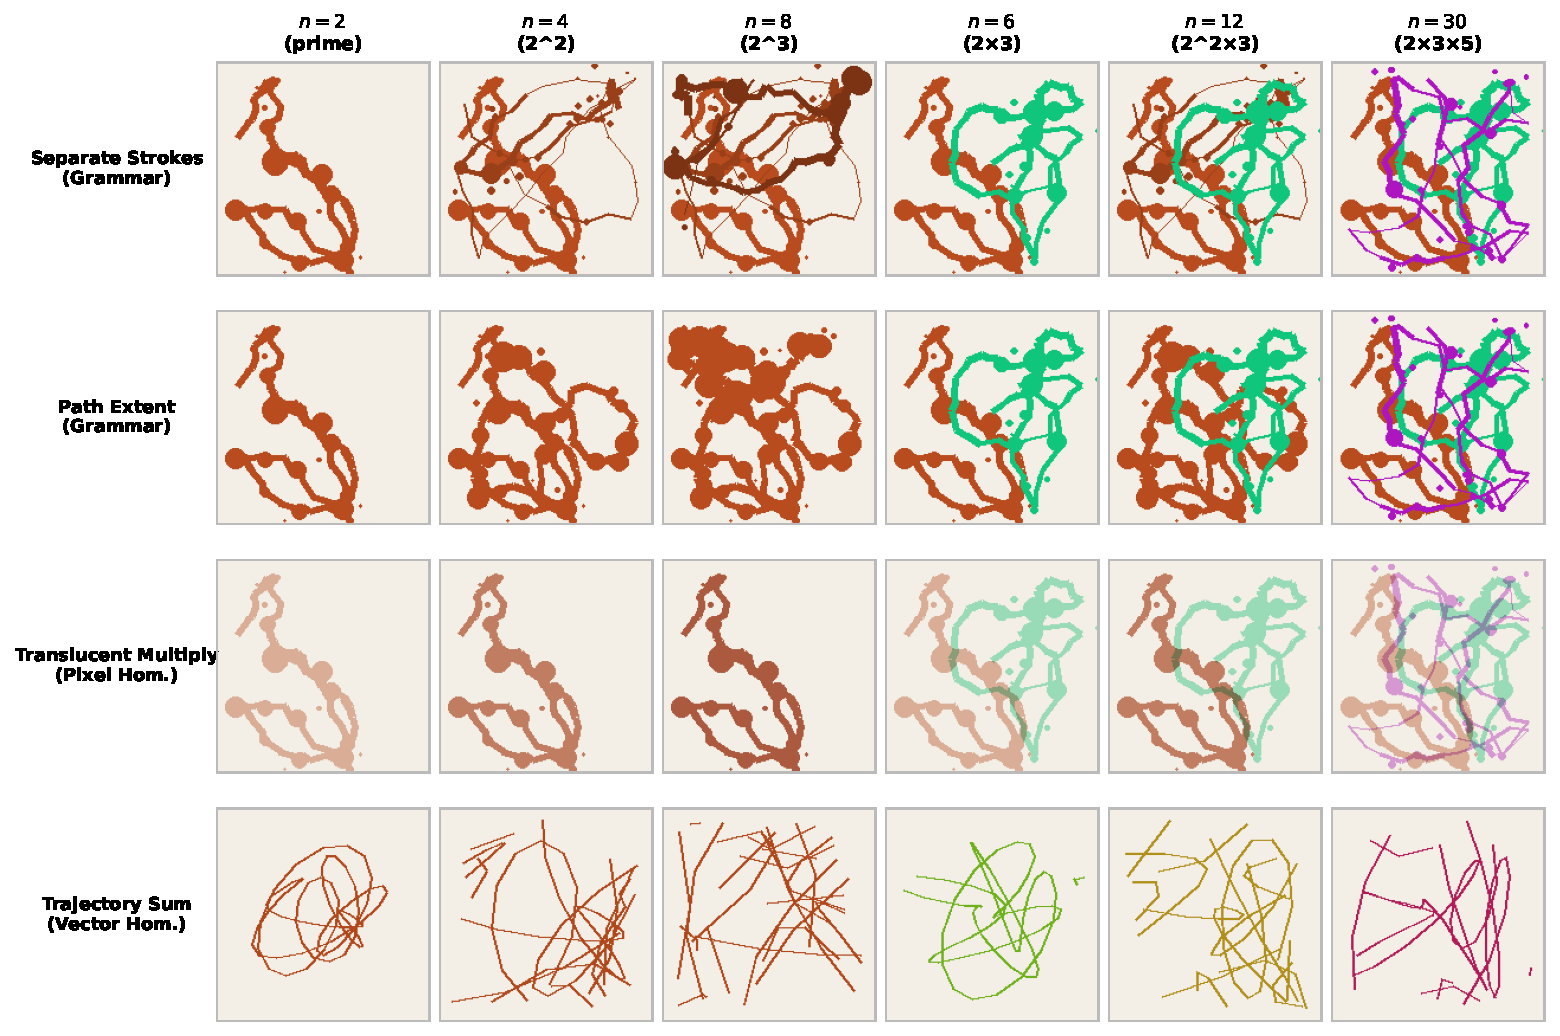
\includegraphics[width=\textwidth]{figures/fig1_pollock_modes.pdf}
  \caption{Comparison of the four multiplicity encodings (rows) across prime powers ($2, 4, 8$) and composites ($6, 12, 30$, columns): two factor-driven generative grammars (top two rows) vs.\ two monoid homomorphisms (bottom two rows).}
  \label{fig:modes}
\end{figure}

\subsection{Generative-Grammar Variants}
In the spirit of \citet{franke1993generative}, where explicit mathematical rules govern generative visual composition, we first define two factor-driven grammars:
\begin{enumerate}
  \item \textbf{Separate Strokes:} For a prime power $p_j^e$, each occurrence $k \in \{1, \dots, e\}$ paints an independent trajectory in $p_j$'s hue with lightness variation $L_0(k) = 42\% - 7\% \cdot ((k - 1) \bmod 3)$, overwriting any underlying pixels opaquely.
  \item \textbf{Path Extent:} For a prime power $p_j^e$, $p_j$ paints a single continuous trajectory by extending the step index in~\eqref{eq:drip_angle}--\eqref{eq:drip_speed} to $t = 1, \dots, e\,T_{\mathrm{base}}$ (so the step count scales linearly as $32e$). Because the PRNG is sequential, the geometric and rasterized trajectory supports prior to occlusion by subsequent primes form a nested, prefix-preserving lineage $\operatorname{supp}(T_{p_j,1}) \subset \operatorname{supp}(T_{p_j,2}) \subset \operatorname{supp}(T_{p_j,3})$.
\end{enumerate}
Like kanji radicals or calligraphic components, these generative grammars preserve immediately legible visual parts, at the cost of requiring the prime-factor multiset $\{p_i^{e_i}\}$ prior to rendering (opaque crossings depend on draw order, and two flat RGB images $I(a), I(b)$ for integers $a, b \in \mathbb{N}_{>0}$ cannot extend shared prime strokes when $\gcd(a,b) > 1$).

\subsection{Homomorphic Variants}
\begin{observation}[TMG Continuous-Space Homomorphism]
Let $\mathcal{I}_{\mathrm{cont}} = \{I \in \mathbb{R}^{S \times S \times 3} : 0 < I \le I_{\mathrm{bg}}\}$ (componentwise) be the space of continuous $S \times S$ RGB images bounded above by a non-zero background image $I_{\mathrm{bg}} \in (0, 1]^{S \times S \times 3}$. Assign each prime $p$ a pixelwise multiplicative RGB transmission factor—called an \emph{attenuation field}—$A_p \in (0, 1]^{S \times S \times 3}$ ($A_p = 1$ outside $p$'s stroke mask, leaving the canvas unchanged, and $A_p = (1 - \alpha) + \alpha C_p$ inside, where $C_p \in (0, 1]^3$ is prime $p$'s normalized RGB color from Section~2 and $\alpha = 0.45 \times 0.88 = 0.396$ is the effective per-coat glaze opacity—combining the $0.88$ stroke opacity with a $0.45$ glazing factor—scaling each RGB channel by a value in $(0, 1]$), and define the \emph{TMG encoding map} $\Phi_{\mathrm{TMG}}(n) = I_{\mathrm{bg}} \odot \prod_p A_p^{v_p(n)}$ over all primes $p$, where $\odot$ is the elementwise Hadamard product and $v_p(n) \ge 0$ is the exponent (multiplicity) of prime $p$ in the factorization of $n$ (with $v_p(n) = 0$ if $p \nmid n$, i.e., the $p$-adic valuation, so $v_p(ab) = v_p(a) + v_p(b)$). Under the pixelwise composition law
\begin{equation}
  I(a) \star I(b) := I_{\mathrm{bg}} \odot \left(\frac{I(a)}{I_{\mathrm{bg}}}\right) \odot \left(\frac{I(b)}{I_{\mathrm{bg}}}\right),
\end{equation}
since $I(a)/I_{\mathrm{bg}}, I(b)/I_{\mathrm{bg}} \in (0, 1]^3$, $\mathcal{I}_{\mathrm{cont}}$ is closed under $\star$, $I_{\mathrm{bg}}$ is the identity, commutativity and associativity follow from componentwise multiplication, so $(\mathcal{I}_{\mathrm{cont}}, \star, I_{\mathrm{bg}})$ is a commutative monoid, and $\Phi_{\mathrm{TMG}}(a \cdot b) = \Phi_{\mathrm{TMG}}(a) \star \Phi_{\mathrm{TMG}}(b)$ holds identically in continuous attenuation space for all $a, b \in \mathbb{N}_{>0}$ (Figure~\ref{fig:hom}, top). Note that the homomorphism property guarantees algebraic compositionality, whereas injectivity is verified numerically only over the finite tested domains.
\end{observation}
Here digital \emph{multiply} blending serves as a mathematical attenuation model inspired by translucent glazes rather than a physical simulation of subtractive Kubelka--Munk pigment mixing.\footnote{The classical Kubelka--Munk optical model \citep{kubelka1931ein} accounts for both spectral light absorption and scattering within physical paint layers, which makes real pigment reflectance nonlinear in layer composition.} Moreover, 8-bit raster quantization $Q(x) = \operatorname{clip}(\operatorname{round}(255x), 0, 255)$ fails to commute with $\star$ ($Q(I(a) \star I(b)) \neq Q(Q(I(a)) \star Q(I(b)))$ in general): across all $306$ unordered pairs\footnote{Counting $\sum_{a=1}^{10} (\lfloor 120/a \rfloor - a + 1) = 306$ pairs; at $100 \times 100 \times 3 = 30{,}000$ RGB channels per image, this yields $306 \times 30{,}000 = 9{,}180{,}000$ channels.} $1 \le a \le b$ with $a \cdot b \le 120$ on $100 \times 100$ 8-bit RGB canvases, the maximum channel discrepancy is $1 / 255$ ($1$ least significant bit, LSB), affecting $89{,}419$ of $9{,}180{,}000$ channels ($0.97\%$).

\begin{observation}[TTS Trajectory-Space Homomorphism]
Each prime $p$ seeds the 32-bit Mulberry32 PRNG to sample a $6$-harmonic parametric curve $\gamma_p : [0, 1] \to \mathbb{R}^2$ in continuous curve parameter $t \in [0, 1]$:
\[
  \gamma_p(t) = \sum_{h=1}^{6} \left( a_{p,h}^{(x)} \cos\!\left(2\pi f_{p,h}^{(x)} t + \phi_{p,h}^{(x)}\right),\; a_{p,h}^{(y)} \sin\!\left(2\pi f_{p,h}^{(y)} t + \phi_{p,h}^{(y)}\right) \right),
\]
summed over harmonic index $h \in \{1, \dots, 6\}$, with independent integer frequencies $f_{p,h}^{(x)}, f_{p,h}^{(y)} \in \{1,\dots,7\}$, independent phases $\phi_{p,h}^{(x)}, \phi_{p,h}^{(y)} \sim \mathcal{U}[0, 2\pi)$, and independent amplitudes $a_{p,h}^{(x)} = (0.13/\sqrt{h})\, u_{p,h}^{(x)}$ and $a_{p,h}^{(y)} = (0.13/\sqrt{h})\, u_{p,h}^{(y)}$ ($u_{p,h}^{(x)}, u_{p,h}^{(y)} \sim \mathcal{U}[0.6, 1.4]$). For any integer $n = \prod_{i=1}^{r} p_i^{e_i}$ (with $\gamma_1(t) \equiv (0, 0)$ for $n=1$), defining the TTS encoding map $\Phi_{\mathrm{TTS}}(n) = \gamma_n$ as a \emph{toroidal trajectory} $\gamma_n : [0, 1] \to \mathbb{T}^2 = \mathbb{R}^2 / \mathbb{Z}^2 \cong [0, 1)^2$ via componentwise modulo-$1$ reduction
\begin{equation}
  \gamma_n(t) \equiv \sum_{i=1}^{r} e_i\,\gamma_{p_i}(t) \pmod{1}
\end{equation}
on the flat $2$-torus \citep{munkres2000topology} realizes the additive prime-exponent composition law as an exact commutative monoid homomorphism $\gamma_{a\cdot b} \equiv \gamma_a + \gamma_b \pmod{1}$ into continuous toroidal trajectory space $\mathcal{T} = C([0,1], \mathbb{T}^2)$ for all $a, b \in \mathbb{N}_{>0}$ (Figure~\ref{fig:hom}, bottom). Injectivity is verified numerically over the finite tested domains rather than proved globally (an integer relation $\sum_i c_i \gamma_{p_i}(t) \equiv 0 \pmod{1}$ is not ruled out analytically).
\end{observation}
In TTS, superscripts $(x)$ and $(y)$ denote the horizontal and vertical coordinate channels of $\gamma_p(t) \in \mathbb{R}^2$. Integer frequencies $f_{p,h}^{(x)}, f_{p,h}^{(y)} \in \{1, \dots, 7\}$ ensure $\gamma_p(0) = \gamma_p(1)$ (closed loops on the torus), while truncating at $6$ harmonics balances organic variety against visual clutter under summation. The base scale $0.13$ gives an RMS excursion of $\approx 0.15$ per coordinate on $[0, 1)$ (scaling inversely with $\sqrt{\sum_{h=1}^{H} 1/h}$ if a different harmonic count $H$ is chosen), preventing small primes from collapsing into a cramped central cluster while relying on toroidal modulo-$1$ wrapping to keep larger sums inside the canvas without nonlinear rescaling. Composites are colored by the $e_i$-weighted circular mean of prime hues and rendered with velocity-coupled width and $4\times$ supersampled RGBA anti-aliasing. Whereas TMG permits direct composition of continuous image representations, TTS requires composition of the underlying parametric trajectories in $\mathcal{T}$ before rasterization, since rasterizing a curve into pixels is nonlinear.

\begin{figure}[t]
  \centering
  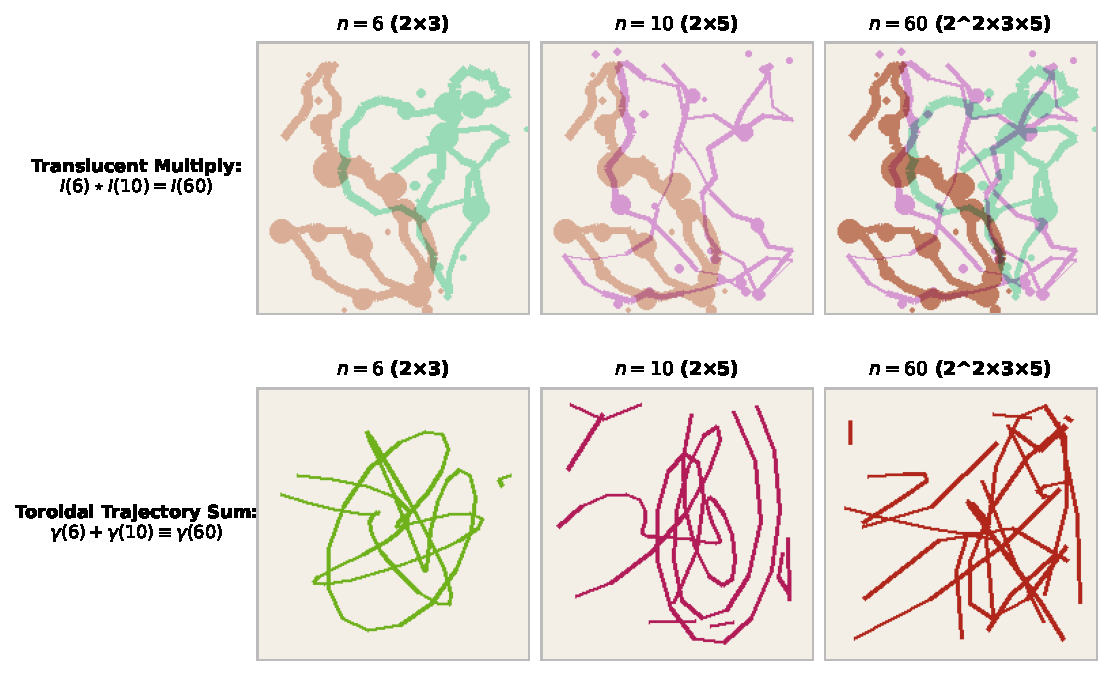
\includegraphics[width=0.92\textwidth]{figures/fig2_pollock_homomorphism.pdf}
  \caption{Direct visual composition $6 \star 10 = 60$ under Translucent Multiply Glazing (TMG, top) and Toroidal Trajectory Sum (TTS, bottom).}
  \label{fig:hom}
\end{figure}

Table~\ref{tab:proscons} summarizes the trade-offs between the two paradigms.

\begin{table}[ht]
  \centering
  \caption{Comparison of Pollock visual homomorphisms and generative grammars.}
  \label{tab:proscons}
  \footnotesize
  \begin{tabular}{@{}p{3.0cm}p{5.1cm}p{5.1cm}@{}}
    \toprule
    Criterion & Visual Homomorphism & Generative Grammar \\
    \midrule
    Composition law & Factor-blind ($\Phi(a) \star \Phi(b)$) & Requires prime multiset $\{p_i^{e_i}\}$ \\
    Exactness domain & Continuous $\mathcal{I}_{\mathrm{cont}}$ (TMG) or $\mathcal{T}$ (TTS) & Discrete raster (order-dependent) \\
    Commutativity & Exact by construction & Requires canonical draw order \\
    Prime powers ($p^e$) & $e$ glazes ($A_p^e$) or $e \cdot \gamma_p$ (toroidal sum) & $e$ strokes or $T_{\mathrm{base}}\cdot e$ path extent \\
    Visual freedom & Constrained by algebra of $\star$ & High (opaque pigments, non-cluttered) \\
    Blind recovery & Glaze peeling or spectrum search & Top-down occlusion peeling \\
    \bottomrule
  \end{tabular}
\end{table}

\section{Visual Uniqueness and Template-Invertibility Recovery}
Once a number is painted, a natural question arises: given only the finished image—without being told which integer it depicts—can we tell every number apart and work backward to identify its prime ingredients? As a proof of concept, we evaluate exact 8-bit RGB-array uniqueness across all $n \in \{1, \dots, 120\}$ and \emph{template-invertibility recovery}—recovering the prime factorization from a raw $100 \times 100$ bitmap using precomputed prime templates and the public rendering rules. Exact-RGB uniqueness is a deterministic digital-array property establishing that no two integers in $\{1, \dots, 120\}$ collide on the $100 \times 100$ raster; it does not imply perceptual distinguishability under arbitrary viewing conditions, compression, or resizing, nor scalability to arbitrary integers. Moreover, because rendering and decoding both require the prime factors or precomputed prime templates, these experiments validate visual invertibility rather than offering an integer-factorization algorithm:

\subsection{Opaque Top-Down Peeling (Separate Strokes)}
Since $(p, k)$ layers are drawn in ascending order, the highest $(p, k)$ present is unoccluded. Scanning $(p, k)$ in descending order, we match unoccluded pixels $U_{p,k} = \operatorname{supp}(T_{p,k}) \setminus \mathcal{O}$ and add $\operatorname{supp}(T_{p,k})$ to the occluded mask $\mathcal{O}$ upon detection.

\subsection{Prefix-Trajectory Peeling (Path Extent)}
Because each distinct prime $p$ draws a single trajectory of $T_{\mathrm{base}} \cdot e$ steps in ascending prime order, scanning primes $p$ from largest to smallest and testing candidate multiplicities $e$ from highest to lowest ($p^e \le 120$) identifies the longest unoccluded prefix $\operatorname{supp}(T_{p,e}) \setminus \mathcal{O}$ present on the canvas, after which $\operatorname{supp}(T_{p,e})$ is added to $\mathcal{O}$.

\subsection{Multiplicative Glaze Peeling (TMG)}
Because multiplicative glaze blending monotonically darkens the normalized ground $R = I / I_{\mathrm{bg}}$, other primes can only decrease $R$; therefore, any $(p, e)$ present satisfies $R(x,y) \le A_p^e(x,y) + \varepsilon$ ($\varepsilon = 0.015 \approx 4$~LSB) at every pixel $(x,y) \in \operatorname{supp}(A_p)$ ($100\%$ of $p$'s support). Across all $p \le 120$, the minimum max-channel separation between $A_p^e$ and $A_p^{e+1}$ is $0.0615$ (at $p=2, e=5 \to 6$), providing a $>4\times$ margin over $\varepsilon$ in isolation (though overlapping primes and quantization-amplified division residuals can still cause misses). Scanning $p$ and $e$ in descending order, a candidate $(p,e)$ is accepted when the inequality holds across $100\%$ of $\operatorname{supp}(A_p)$ and is divided out via $R \leftarrow \min(1, R / A_p^e)$ (Figure~\ref{fig:peeling}).

\subsection{Prime-Spectrum Search (TTS)}
Using only the $30$ prime Fourier curves $\{\gamma_p\}_{p \le 120}$, depth-first search over non-decreasing prime products $\prod p_i^{e_i} \le 120$ matches the rendered bitmap without storing any composite table. Counting each candidate composite render and $S \times S$ pixel comparison, the peeling decoders (4.1--4.3) run in $O(\pi(N) \log N \cdot S^2)$ pixel operations, whereas TTS search explores $O(N)$ prime-product branches in $O(N \cdot \pi(N) \cdot S^2)$ worst-case pixel operations (without caching).

\begin{figure}[t]
  \centering
  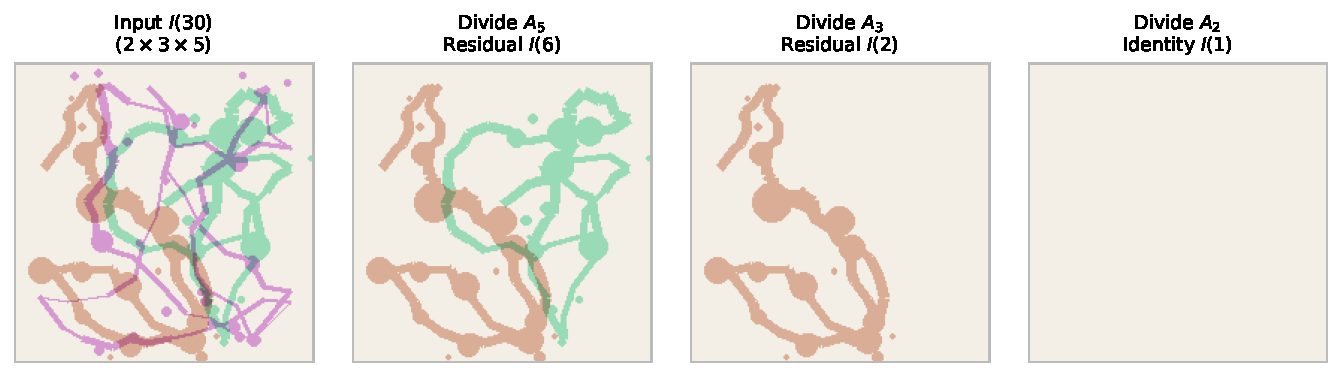
\includegraphics[width=0.95\textwidth]{figures/fig3_pollock_peeling.pdf}
  \caption{Blind multiplicative glaze peeling of $n = 30 = 2 \times 3 \times 5$ in Pollock Translucent Multiply Glazing (TMG) mode.}
  \label{fig:peeling}
\end{figure}

Across all $120$ integers $n \in \{1, \dots, 120\}$ at $100 \times 100$ RGB, all four Pollock variants produce $120$ out of $120$ ($100\%$) exact-RGB unique images and $120$ out of $120$ ($100\%$) template-invertibility recoveries ($0$ errors), with $0$ homomorphism errors in continuous 32-bit floating-point attenuation space (TMG) and continuous trajectory space (TTS) across all $a \cdot b \le 120$\footnote{In continuous space, $\Phi_{\mathrm{TMG}}(a \cdot b) = \Phi_{\mathrm{TMG}}(a) \star \Phi_{\mathrm{TMG}}(b)$ and $\Phi_{\mathrm{TTS}}(a \cdot b) = \Phi_{\mathrm{TTS}}(a) \star \Phi_{\mathrm{TTS}}(b)$ hold identically at any canvas resolution by construction; the discrete check verifies numerical agreement across all tested $S$.}. In an image-size ablation across $64 \times 64$, $128 \times 128$, and $256 \times 256$ canvases (testing whether lower spatial resolution increases raster collisions or breaks peeling tolerances), all four variants likewise retain $100\%$ uniqueness ($120$ out of $120$), $100\%$ recovery, and $0$ continuous homomorphism errors at every tested resolution (with $O(S^2)$ decoding cost). Extending beyond $n \le 120$ on $200$ random integers in $2 \dots 10{,}000$ ($100 \times 100$), Separate Strokes, Path Extent, and TMG all achieve $200/200$ ($100.0\%$) recovery, while TTS achieves $500/500$ ($100.0\%$) uniqueness, $500/500$ recovery, and $0$ continuous trajectory-space homomorphism errors across all $n \le 500$. To probe higher prime-factor counts for TMG—the variant adopted in the Section~\ref{sec:codec} message codec—we tested an initial sample of $4$--$7$ prime primorials ($210, 2310, 30030, 510510$) and $100$ random composites $n \le 10^6$ with prime factors $\le 1000$: TMG recovered $4/4$ primorials and $99/100$ random composites at both $100 \times 100$ and $256 \times 256$; the single failure in both cases was $n = 432{,}162 = 2 \cdot 3^3 \cdot 53 \cdot 151$, where the small prime $p = 2$ ($e = 1$) was missed after dividing out the heavily overlapping $151$, $53$, and $3^3$ glazes under 8-bit quantization, leaving a residual pixel above the $\varepsilon = 0.015$ threshold. Grouping an independent $250$-composite stress sample ($n \le 10^6$, $50$ random composites for each number of distinct prime factors $r \in \{2, 3, 4, 5, 6\}$ on $100 \times 100$-pixel canvases) yields $50/50$ ($100.0\%$) recovery in every bin, suggesting that failures are uncommon in the tested configurations and are associated with quantization artifacts near the detection tolerance.

\section{Single-Canvas Message Encoding and Geometric Resilience}
\label{sec:codec}
The same prime-indexed attenuation mechanism can also encode binary information: instead of interpreting prime exponents as multiplicities in an integer factorization, we restrict them to binary values $b_j \in \{0, 1\}$, with each prime indicating the presence or absence of one message bit on a unified $512 \times 512$ canvas. Specifically, we map a $K$-bit UTF-8 binary string (most-significant-bit first) to primes $p_0, \dots, p_{K-1}$ ($2, 3, 5, \dots$), rendering each active prime under TMG with $\alpha = 0.50$ in $A_p = (1 - \alpha) + \alpha C_p$, shorter and thinner strokes, a $10\%$ margin, and hues excluding $C_{T_0}$ (constants in \texttt{report\_all\_modes.pdf}). Because binary payloads restrict exponents to $\{0,1\}$ (unlike the unrestricted TMG monoid, where overlapping active primes sum to multiplicity $2$), the binary codec uses TMG's attenuation mechanism as a restricted subset closed under TMG composition only on disjoint active prime-index sets. Because trailing zero bits omit their trajectories, the current unframed protocol assumes a fixed payload length $K$ known to the decoder (e.g., $K \in \{64, 127, 128\}$). For an illustrative example string such as \texttt{"MathArts"} ($8$ UTF-8 bytes, $64$ bits, shown in Figure~\ref{fig:leonardo_rts}), only the first $64$ primes ($2 \dots 311$) are needed.

\subsection{Keyed Organic Registration Skein and Log-Attenuation Decoding}
To align rotated, translated, and scaled (RTS) canvases without external finder squares or corner dots that would disrupt the artistic composition, we paint an \emph{integrated registration pattern} (opaque top-skein $T_0$, a registration/finder pattern inset by a $12\%$ margin) on top of the glazed data strokes. Both the PRNG seed and pigment color of $T_0$ are parameterizable: a default public seed (Venetian crimson) enables open decoding, whereas an artist-chosen seed and color (e.g., Ultramarine or Forest Viridian) yield distinct visual compositions and act as a keyed registration template. During decoding:
\begin{enumerate}
  \item A soft chromatic response map $M(x,y) = \exp(-\|I(x,y) - C_{T_0}\|_2^2 / 30^2)$ isolates $T_0$ from the distorted canvas on a $0.25\times$ downsampled grid ($128 \times 128$): it scores each pixel's RGB similarity to $C_{T_0}$ smoothly on $[0, 1]$ (Gaussian color tolerance $\sigma = 30$ RGB levels), keeping pixels near $C_{T_0}$ bright while fading out the cream background and data strokes without brittle hard thresholding that would clip blurred edges.
  \item \emph{Fourier--Mellin registration} \citep{reddy1996fft,oruanaidh1997rotation} resamples the high-pass FFT magnitude spectra onto a log-polar grid and applies phase correlation to obtain a coarse rotation and scale estimate across $[0.80, 1.20]$; both $\theta$ and $\theta + 180^\circ$ (with $\pm$ signs and reciprocal scale checks) are then disambiguated and locally refined via normalized Cartesian FFT cross-correlation ($0.25^\circ$ angular steps and $0.7\%$--$0.8\%$ scale steps spanning $\pm 1.5\%$), followed by a full-resolution ($512 \times 512$) FFT translation polish.
  \item Masking out $T_0$, taking the negative logarithm of the normalized ground converts multiplicative glazing into a linear model in log-attenuation space:
  \[
    L_{\mathrm{obs}}(x,y) := -\log\!\left(\frac{I_{\mathrm{aligned}}(x,y)}{I_{\mathrm{bg}}}\right) \approx \sum_{j=0}^{K-1} b_j\, L_j(x,y),
  \]
  where each unnormalized binary-support template vector $L_j \in \mathbb{R}^{3S^2}$ equals $-\log((1-\alpha) + \alpha C_{p_j}) \in \mathbb{R}^3$ at every unoccluded stroke pixel $(x,y) \in \operatorname{supp}(p_j) \setminus \operatorname{supp}(T_0)$ across all three RGB channels, and $\mathbf{0}$ elsewhere. In the ideal continuous attenuation model, the logarithm converts multiplicative composition into exact addition; after geometric resampling—where bilinear interpolation averages RGB values before the logarithm, $-\log(\sum_i w_i I_i) \neq \sum_i w_i [-\log(I_i)]$—and 8-bit quantization, the system is approximate and is solved via ridge-regularized least squares $\min_{\mathbf{b}} \|L_{\mathrm{obs}} - \sum_{j=0}^{K-1} b_j L_j\|_2^2 + \lambda \|\mathbf{b}\|_2^2$, yielding $(G + \lambda I_K)\hat{\mathbf{b}} = \mathbf{y}$ with $G_{jl} = \langle L_j, L_l \rangle$, $y_j = \langle L_j, L_{\mathrm{obs}} \rangle$, $\lambda = 10^{-3}$, and bit decision $\hat{b}_j \ge 0.5$.
\end{enumerate}

The opaque top-skein $T_0$ occupies only $3.35\%$ of the $512 \times 512$ canvas, occluding on average $4.72\%$ (median $4.22\%$, max $15.43\%$) of each prime template's pixels for $K = 64$ and $4.94\%$ (median $4.34\%$, max $18.54\%$) for $K = 128$. Masking $T_0$ leaves the Gram matrix $G = A^\top A$ nearly unchanged and well-conditioned: at $512 \times 512$, its $2$-norm condition number\footnote{With $A = [L_0 \mid \dots \mid L_{K-1}] \in \mathbb{R}^{3S^2 \times K}$ denoting the column-stacked template matrix ($L_{\mathrm{obs}} \approx A\mathbf{b}$), the normal equations use the Gram matrix $G = A^\top A$. Since the columns $L_j$ are linearly independent, $\kappa_2(G) = \lambda_{\max}(G)/\lambda_{\min}(G) = \kappa_2(A)^2$ (so $\kappa_2(A) \approx 2.64$ for $K=64$ and $3.37$ for $K=128$); we report $\kappa_2(G)$ because $(G + \lambda I_K)\hat{\mathbf{b}} = \mathbf{y}$ is the $K \times K$ linear system actually solved during decoding.} is $\kappa(G) = 6.95$ for $K = 64$ (vs.\ $6.86$ unmasked; mean off-diagonal correlation $0.033$, max $0.142$) and $\kappa(G) = 11.37$ for $K = 128$ (vs.\ $11.32$ unmasked; mean $0.033$, max $0.170$). Compared with the orthogonal ideal $\kappa = 1$ and ill-conditioned regimes ($\kappa \gg 10^4$), these values near $10$ lose only $\sim 1$ decimal digit in IEEE-754 double-precision arithmetic, ensuring that the compact $K \times K$ normal-equations solve is numerically well-behaved for this problem without needing a full $(3S^2) \times K$ QR or SVD decomposition. Because $\lambda_{\min}(G) \approx 30$, $\lambda = 10^{-3}$ acts purely as a conservative numerical safeguard: a sensitivity sweep on $200$ trials of $128$-bit RTS + JPEG ($q=80$) across $\lambda \in \{0\text{ (OLS)}, 10^{-5}, 10^{-4}, 10^{-3}, 10^{-2}, 10^{-1}\}$ yields identical $177/200$ ($88.5\%$) exact-message recovery and $99.77\%$ bit accuracy for every tested $\lambda$.

\begin{figure}[t]
  \centering
  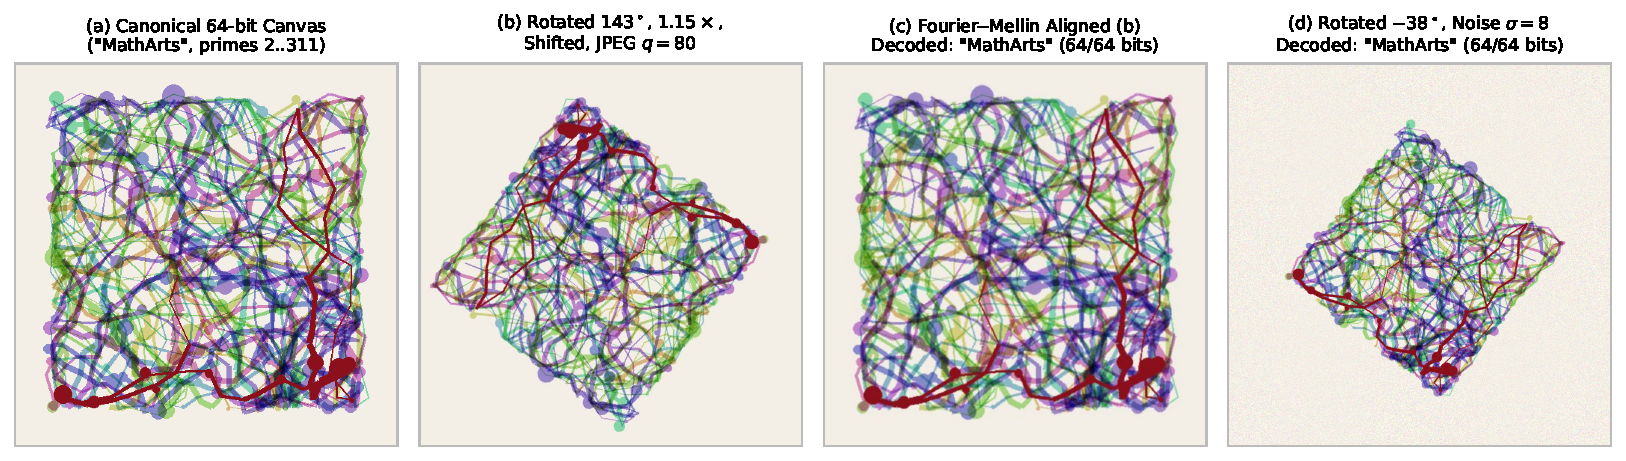
\includegraphics[width=\textwidth]{figures/fig4_pollock_matharts_rts.pdf}
  \caption{Single-canvas $64$-bit encoding of \texttt{"MathArts"} (primes $2 \dots 311$, $512 \times 512$, organic top-skein): (a) canonical canvas; (b) rotated $143^\circ$, scaled $1.15\times$, shifted, and JPEG-compressed ($q=80$); (c) Fourier--Mellin aligned (b), decoded ($64/64$ bits); (d) rotated $-38^\circ$, $0.95\times$, shifted, with Gaussian noise ($\sigma=8$), decoded ($64/64$ bits).}
  \label{fig:leonardo_rts}
\end{figure}

\subsection{Statistical Evaluation, Registration Accuracy, and Comparison}
Figure~\ref{fig:leonardo_rts} illustrates $64/64$ bit recovery for the example string \texttt{"MathArts"} on the canonical canvas and under two combined distortions (with (c) showing the aligned recovery of (b)), and changing the keyed top-skein to Ultramarine or Forest Viridian likewise achieves $64/64$ recovery under $143^\circ$ RTS + JPEG ($q=80$). To quantify statistical reliability beyond a single message, Table~\ref{tab:rts} reports $1{,}000$-trial Monte Carlo benchmarks for random $64$-bit and $128$-bit payloads. Using a fixed PRNG seed (documented in the companion technical report and code, with independent $1{,}000$-trial runs for $K=64$ and $K=128$), each trial generates an independent random $K$-bit payload and independent transformation parameters $\theta \sim \mathcal{U}[-180^\circ, 180^\circ]$, $s \sim \mathcal{U}[0.80, 1.20]$, and $(\Delta x, \Delta y) \sim \mathcal{U}[-20, 20]^2$~px, evaluating the same payload and transform sample under both JPEG ($q=80$) and Gaussian noise ($\sigma=8$). The $512 \times 512$ canvas is padded by $25\%$ ($128$~px) on each side to $768 \times 768$ ($1.50S \times 1.50S$) before bilinear rotation/scaling; including the $\pm 20$~px shift, $1.20 \times 0.80\sqrt{2} \times 512 + 2(20) = 735.3 < 768$, so the $10\%$ data margin and $12\%$ top-skein margin guarantee zero clipping of painted strokes across all tested angles, scales, and shifts, and pixel values are clipped to $[0, 255]$ after noise:
\begin{itemize}
  \item \textbf{Registration accuracy and error source isolation:} Across all $1{,}000$ degraded trials ($128$-bit), Fourier--Mellin alignment achieves mean absolute rotation error $0.149^\circ \pm 0.114^\circ$ (JPEG $q=80$) and $0.143^\circ \pm 0.109^\circ$ (noise $\sigma=8$), with scale error $0.0050 \pm 0.0035$ and $0.0050 \pm 0.0036$ (matching the $0.7\%$--$0.8\%$ scale grid). On the $200$-trial $128$-bit RTS + JPEG ($q=80$) subset, there are $0/200$ catastrophic registration failures: rotation error has mean $0.150^\circ$, $95$th percentile $0.369^\circ$, and max $0.530^\circ$, while scale error has mean $0.0050$, $95$th percentile $0.0119$, and max $0.0158$; residual scale error correlates strongly with per-trial bit errors ($r = 0.591$), whereas residual rotation error does not ($r = -0.046$). A $200$-trial $128$-bit isolation ablation shows $200/200$ ($100.00\%$ bits) for JPEG-only ($q=80$) and $200/200$ ($100.00\%$ bits) for noise-only ($\sigma=8$), versus $178/200$ ($89.0\%$ msgs, $99.70\%$ bits, $0.38 \pm 1.35$ err; within sampling variability of the $1{,}000$-trial RTS+JPEG/noise bit accuracies of $99.74\%$--$99.76\%$, whose $95\%$ CIs overlap) for RTS-only (without JPEG compression or added noise)—confirming that geometric resampling blur and residual misalignment drive virtually all bit errors. Single-threaded decode latency on $100$ trials averages $106.7 \pm 2.7$~ms (clean), $161.4 \pm 8.9$~ms (RTS+JPEG80), and $162.4 \pm 9.6$~ms (RTS+Noise8).
  \item \textbf{Coefficient separation, error distribution, and BCH error correction:} Under $128$-bit RTS + JPEG ($q=80$), all true $0$-bits remain below threshold ($\max \hat{b}_j = 0.418 < 0.5$, $95$th percentile $0.288$), so all errors are $1 \to 0$ attenuation drops from resampling blur; the $5$th percentile of the \emph{per-trial minimum} $\min_{j: b_j=1} \hat{b}_j$ is $0.442$ (global min $0.303$). Across $1{,}000$ trials, bit accuracy is $99.76\%$ (trial-level cluster-adjusted $95\%$ CI $\hat{p} \pm 1.96\,s_{\mathrm{err}}/(K\sqrt{1000}) = [99.71\%, 99.81\%]$, where each trial is an independent statistical unit and $s_{\mathrm{err}}$ is the sample SD of the per-trial bit-error counts), while $12.3\%$ of uncoded $128$-bit messages have $\ge 1$ error ($99.0\%$ have $\le 5$ errors, max $9$ for JPEG and $11$ for noise; full error-count histograms are given in \texttt{report\_all\_modes.pdf} in the repository). For $64$-bit payloads under RTS + JPEG ($q=80$), exact-message recovery is $92.3\%$ ($95\%$ CI $[90.5\%, 93.8\%]$, max $6$ errors). In a separate $400$-trial experiment with a $92$-bit payload ($11$ UTF-8 bytes plus $4$ zero-pad bits) encoded via systematic $\mathrm{BCH}(127, 92, t=5)$ over $\mathrm{GF}(2^7)$ onto $127$ primes ($2 \dots 709$), the decoder corrects up to $5$ bit errors and flags codewords with $>5$ errors as uncorrectable: exact-message recovery rises from $343/400$ ($85.75\%$) to $396/400$ ($99.00\%$, $99.954\%$ bit accuracy; $4$ uncorrectable $>5$-error trials) under RTS + JPEG ($q=80$) and from $342/400$ ($85.50\%$) to $396/400$ ($99.00\%$, $99.943\%$ bit accuracy; $4$ uncorrectable trials) under RTS + noise ($\sigma=8$).
\end{itemize}

\begin{table}[ht]
  \centering
  \caption{Single-canvas recovery across $512 \times 512$ Pollock distortion regimes ($1{,}000$-trial Monte Carlo for $64$-bit and $128$-bit payloads; $95\%$ Wilson confidence intervals for exact-message and zero-error clean bit rates, and trial-level cluster-adjusted $95\%$ CIs for degraded bit accuracy).}
  \label{tab:rts}
  \footnotesize
  \begin{tabular}{@{}llll@{}}
    \toprule
    Payload \& Scenario & Exact Msgs ($95\%$ CI) & Bit Acc.\ ($95\%$ CI) & Bit Err (Max) \\
    \midrule
    \multicolumn{4}{@{}l}{\emph{64-bit Random Payloads ($1{,}000$ trials, $64{,}000$ bits/regime)}} \\
    Clean canonical & $1000/1000$ ($100.0\%$, $[99.6,100.0]$) & $100.00\%$ ($[99.99,100.00]$) & $0.00 \pm 0.00$ ($0$) \\
    RTS + JPEG $q=80$ & $923/1000$ ($92.3\%$, $[90.5,93.8]$) & $99.76\%$ ($[99.70,99.82]$) & $0.15 \pm 0.65$ ($6$) \\
    RTS + noise $\sigma=8$ & $924/1000$ ($92.4\%$, $[90.6,93.9]$) & $99.76\%$ ($[99.70,99.82]$) & $0.15 \pm 0.65$ ($6$) \\
    \addlinespace
    \multicolumn{4}{@{}l}{\emph{128-bit Random Payloads ($1{,}000$ trials, $128{,}000$ bits/regime)}} \\
    Clean canonical & $1000/1000$ ($100.0\%$, $[99.6,100.0]$) & $100.00\%$ ($[100.00,100.00]$) & $0.00 \pm 0.00$ ($0$) \\
    RTS + JPEG $q=80$ & $877/1000$ ($87.7\%$, $[85.5,89.6]$) & $99.76\%$ ($[99.71,99.81]$) & $0.31 \pm 1.05$ ($9$) \\
    RTS + noise $\sigma=8$ & $873/1000$ ($87.3\%$, $[85.1,89.2]$) & $99.74\%$ ($[99.69,99.80]$) & $0.33 \pm 1.15$ ($11$) \\
    \bottomrule
  \end{tabular}
\end{table}

To contextualize information density against conventional 2D machine codes, a $21 \times 21$ Version-1 QR code at Error Correction Level~L ($136$ usable byte-mode payload bits) rendered at $512 \times 512$ pixels has density $5.2 \times 10^{-4}$~usable bits/pixel (comparable to our $\mathrm{BCH}(127, 92)$ coded density of $92 / 512^2 \approx 3.51 \times 10^{-4}$~bits/pixel), whereas a Version-40 QR code reaches $\sim 0.09$~bits/pixel ($\sim 185\times$ denser than our uncoded $128$-bit rate). This illustrative comparison highlights that our design is not intended to compete on raw capacity with dedicated machine barcodes, but rather trades density for full aesthetic integration without artificial finder squares. Moreover, because the encoded trajectories are visible and any party knowing the rendering rules and top-skein seed can reconstruct the $K$ templates and solve the same linear log-attenuation system ($\mathbf{b} \mapsto L_{\mathrm{obs}}$), the system is a \emph{visible artistic visual code} rather than a cryptographic or steganographic primitive.

\section{Limitations}
Several practical boundaries bound the current framework:
\begin{enumerate}
  \item \textbf{Capacity and stroke crowding:} As $K$ grows beyond $128$ primes on a $512 \times 512$ canvas ($4.88 \times 10^{-4}$~bits/pixel), inter-prime stroke overlap increases Gram-matrix conditioning $\kappa(G)$ and raises attenuation crowding, requiring larger canvases or thinner filaments.
  \item \textbf{Geometric warp model:} Fourier--Mellin registration handles planar similarity transforms within the tested scale range $[0.80, 1.20]$; severe perspective skew, non-uniform aspect-ratio stretching, or heavy cropping/occlusion of the registration skein $T_0$ would require projective registration.
  \item \textbf{Chromatic and quantization sensitivity:} Both the top-skein response map $M(x,y)$ and log-attenuation decoding assume calibrated RGB white balance and gamma, and 8-bit quantization introduces $\pm 1$ LSB rounding differences ($0.97\%$ of channels in TMG); physical print-and-photograph capture remains untested.
  \item \textbf{Seed dependence and security:} Opaque peeling and linear decoding depend on the chosen PRNG seeds and lack cryptographic secrecy unless $T_0$'s seed is kept private as a keyed watermark.
  \item \textbf{Precomputation cost:} Decoding precomputes $K$ prime stroke templates and $(G + 10^{-3}I_K)^{-1}$ once per keyset, scaling as $O(K^2 S^2)$ for Gram-matrix construction and $O(K^3)$ for matrix inversion (though a direct linear solve avoids explicit inversion).
  \item \textbf{Finite-domain validation:} The $100\%$ ($120$ out of $120$) uniqueness and factor-recovery results verify the constructions over $1 \le n \le 120$ and do not establish scalability to arbitrary integers; the larger-domain TMG experiments remain preliminary.
  \item \textbf{Perceptual and physical validation:} All representations are evaluated computationally on synthetic rasters; neither human perceptual studies nor physical print-and-photograph capture have yet been conducted.
  \item \textbf{Payload framing and length recovery:} Because trailing inactive primes produce no visual strokes, the current codec assumes a fixed payload length $K$ known to the decoder; variable-length messages would require an explicit length header.
\end{enumerate}

\section{Conclusion}
Focusing on Jackson Pollock's drip-painting aesthetic demonstrates that visual number representations can bridge formal algebra and expressive art. While generative grammars (\emph{Separate Strokes} and \emph{Path Extent}) prioritize clear, layered silhouettes, Translucent Multiply Glazing (TMG) realizes an exact commutative monoid homomorphism in continuous attenuation fields (with at most a $1$-LSB discrepancy in the tested 8-bit RGB compositions), and Toroidal Trajectory Sum (TTS) realizes an exact homomorphism in continuous toroidal trajectory space $\mathcal{T} = C([0,1], \mathbb{T}^2)$. As a proof of concept over $1 \le n \le 120$, all four variants achieve $100\%$ exact-RGB uniqueness and template-invertibility recovery, with $200/200$ recovery extending up to $n \le 10{,}000$ for Separate Strokes, Path Extent, and TMG, and $500/500$ for TTS up to $n \le 500$. Extending TMG to single-canvas message encoding with a keyed organic registration template yields $64/64$ bit recovery in the \texttt{"MathArts"} demonstration, $99.74\%$--$99.76\%$ bit accuracy ($87.3\%$--$92.4\%$ uncoded exact messages) across $1{,}000$-trial Monte Carlo benchmarks, and $99.00\%$ exact-message recovery with $\mathrm{BCH}(127, 92, t=5)$ error correction. More broadly, this framework shows how abstract algebraic composition laws can be embedded directly into expressive visual media, opening possibilities beyond prime-factor visualization.

\section*{Code and Data Availability}
The complete Python implementation (\texttt{verify\_decomposition.py}, \texttt{pollock\_codec.py}), interactive HTML/Canvas/SVG explorer (\texttt{build\_explorer.py}, \texttt{explorer.html}, including the Text/Binary/Hex-to-Art codec tab), and figure-generation scripts are publicly available at \url{https://github.com/leolca/prime_visual_algebra} (revised submission state, using a direct linear solve via \texttt{np.linalg.solve} in \texttt{pollock\_codec.py}). All experiments were executed with Python~3.14.8, NumPy~2.4.6, and Pillow~12.3.0 on an Intel Core i7-13650HX CPU; \texttt{python3 verify\_decomposition.py} reproduces the Section~4 verification checks and \texttt{python3 pollock\_codec.py} reproduces the \texttt{"MathArts"} demonstration.

\section*{Disclosure Statement}
The author reports there are no competing interests to declare.

\section*{Funding}
This research received no external funding.

\bibliographystyle{tfapacite}
\bibliography{references}

\end{document}
